% Mathe Formelsammlung für HM1 ZHAW
% 2 Seiten


% Dokumenteinstellungen
% ======================================================================

% Dokumentklasse (Schriftgröße 6, DIN A4, Artikel)
\documentclass[8pt,a4paper]{scrartcl}

% Zusätzliche Pakete laden
\usepackage[utf8]{inputenc}        % Zeichenkodierung: UTF-8 (für Umlaute)
\usepackage[german]{babel}        % Deutsche Sprache
\usepackage{multicol}            % Spaltenpaket
\usepackage{amsmath}            % erlaubt mathematische Formeln
\usepackage{amssymb}            % Verschiedene Symbole
\usepackage{esint}                % erweiterte Integralsymbole
\usepackage{booktabs}            % bessere Tabellenlinien
\usepackage{graphicx}            % Zum Bilder einfügen benötigt
\usepackage{color}                % Farbiger Text möglich
\usepackage{pbox}                % Intelligent parbox: \pbox{maximum width}{blabalbalb \\ blabal}
%\usepackage{undertilde}            % Für Welle unterhlab von Matrixbuchstaben benötigt
\usepackage{accents}            % Für eigene Ableitungspunkte benötigt
\usepackage{scrtime}
\usepackage{supertabular}        % Für lange Tabellen mit Umbruch
\usepackage{pdfpages}
\usepackage{trfsigns}            % Laplace und Fourier
\usepackage{array}


% Seitenlayout und Ränder:
\usepackage{geometry}
\geometry{a4paper,landscape, left=6mm,right=6mm, top=-1mm, bottom=3mm,includeheadfoot}
\setlength{\parindent}{0mm}


% Dokumentbeschreibung
\title{Formelsammlung Höhere Mathematik 1 ZHAW}
\author{Andreas Sprecher}


% Kopf- und Fußzeile
% ======================================================================
\usepackage{fancyhdr}
\pagestyle{fancy}
\fancyhf{}
   \fancyfoot[C]{\textbf{Statistik}}
   \renewcommand{\headrulewidth}{0.0pt} %obere Linie ausblenden
   \renewcommand{\footrulewidth}{0.1pt} %obere Linie ausblenden

   \fancyfoot[R]{Stand: \todayV}
   \fancyfoot[L]{Andreas Sprecher}
% ----------------------------------------------------------------------

% Ausgegraut zum Abschreiben:
%\definecolor{grey}{rgb}{0.6,0.6,0.6}
%\color{grey}

% Befehle und Befehlsüberschreibungen
% ======================================================================

% Schriftart SANS für bessere Lesbarkeit bei kleiner Schrift
\renewcommand{\familydefault}{\sfdefault}
% Array- und Tabellenabstände vergrößern
\renewcommand{\arraystretch}{1.2}

% Befehle sichern
\let\oldvec = \vec
\let\olddot = \dot

% Eigene Befehle
\newcommand{\todayV}{\the\day.\the\month.\the\year}                          %%D.M.YYYY

\newcommand{\iset}[2]{\ensuremath{\bigl\{ \bigl. #1 \, \bigr| \, #2 \bigr\}}}                   % intensional set
\newcommand{\eset}[1]{\ensuremath{\bigl\{#1\bigr\}}}                                            % extensional set
%\newcommand{\enbrace}[1]{\ensuremath{\bigl\(#1\bigr\)}}                                        % extensional set
\newcommand{\enbrace}[1]{\ensuremath{\left(#1\right)}}
\newcommand{\norm}[1]{\ensuremath{\|#1\|}}                                                      % Norm
\newcommand{\mat}[1]{\ensuremath{\begin{bmatrix} #1 \end{bmatrix}}}                             % Matrix
\newcommand{\ma}[1]{\ensuremath{\boldsymbol {#1}}}                                              % Matrixsymbol
\newcommand{\vect}[1]{\ensuremath{\begin{pmatrix} #1 \end{pmatrix}}}                            % Vektor
\newcommand{\mvect}[1]{\ensuremath{\left. \begin{matrix} #1 \end{matrix}  \right]}}             % Matrixvektornotation
\newcommand{\gk}[1]{\ensuremath{\left\lfloor#1\right\rfloor}}                                   % Gaußklammer
\newcommand{\sprod}[2]{\ensuremath{\left\langle #1, #2 \right\rangle }}                         % Skalarprodukt
\newcommand{\abs}[1]{\ensuremath{\left\vert#1\right\vert}}                                      % Betrag
\newcommand{\bdot}{\ensuremath{\boldsymbol \cdot}}                                              % Dicker Punkt für Skalarprodukt
\newcommand{\svdots}{\ensuremath{\olddot :}}                                                    % small vertical dots
\newcommand{\mustbe}{\stackrel{!}{=}}

\newcommand{\inn}{\operatorname{int}}


% Überschreibungen
\renewcommand{\vec}[1]{\ensuremath{\boldsymbol {#1}}}                                           % Vektor fett und unterstrichen
\renewcommand{\emph}[1]{\textbf{#1}}                                                            % Hervorhebungen fett
\renewcommand*{\dot}[1]{\accentset{\mbox{\textrm{\large\bfseries .}} }{#1}}                     % Dicker Ableitungspunkt
\renewcommand*{\ddot}[1]{\accentset{\mbox{\textrm{\large\bfseries .\hspace{-0.25ex}.}}}{#1}}    % Dicker Doppelableitungspunkt

% Abkürzungen
\newcommand{\ul}[1]{\ensuremath{\underline{#1}}}                               % Untersteichen
\newcommand{\ol}[1]{\ensuremath{\overline{#1}}}                                % Überstreichen
\newcommand{\Ra}[0]{\ensuremath{\Rightarrow}}                                  % Rightarrow
\newcommand{\ra}[0]{\ensuremath{\rightarrow}}                                  % Rightarrow
\newcommand{\bs}[1]{\ensuremath{\boldsymbol{#1}}}                              % Fett und kursiv im mathmode
\newcommand{\diff}{\ensuremath{\;\mathrm d}}                                   % differentielles delta
\newcommand{\grad}{\ensuremath{\mathrm{grad}\ }}                               % Gradient
\renewcommand{\div}{\ensuremath{\mathrm{div}\ }}                               % Divergenz
\newcommand{\rot}{\ensuremath{\mathrm{rot}\ }}                                 % Rotation
\newcommand{\Sp}{\ensuremath{\mathrm{Sp}\ }}                                   % Spur
\renewcommand{\i}{\ensuremath{\mathrm{i}}}                                     % Imaginäre Einheit

% Für Mengen
\newcommand{\N}{\ensuremath{\mathbb N}}
\newcommand{\R}{\ensuremath{\mathbb R}}
\newcommand{\C}{\ensuremath{\mathbb C}}


%Custom functions
\DeclareMathOperator{\arccot}{arccot}
\DeclareMathOperator{\Kern}{kern}
\DeclareMathOperator{\rang}{rang}
\DeclareMathOperator{\col}{col}
\DeclareMathOperator{\row}{row}


% Dokumentbeginn
% ======================================================================
\begin{document}


% Aufteilung in Spalten
\begin{multicols*}{3}
\setlength{\columnseprule}{0.4pt}
    \parbox{3cm}{
        \includegraphics[height=1.5cm]{./img/Logo.jpeg}
    }
    \parbox{4cm}{
        \emph{\Large{Statistik}}
    }
    \vspace{-2mm} 

    \section{Deskriptive Statistik}
    		\subsection{Merkmalstypen}
    			\subsubsection{Qualitativ/Kategoriell}
    				Endliche Anzahl Ausprägungnen
    				\begin{itemize}\itemsep0pt				
					\item Nominal (Kategorisierung, keine Ordnung)
					\item Ordinal (Ranggierung möglich, Ordnung möglich)
				\end{itemize}
    			\subsubsection{Quantitativ/Metrisch}
    				Ausmass in Zahlen
    				\begin{itemize}\itemsep0pt				
					\item Diskret (Fixe Sprunggrösse)
					\item Stetig (Reelle Sprunggrösse)
				\end{itemize}
		\subsection{PDF \& CDF}
			Vorkommnis: 1, 2, 3 \\
			Häufigkeit: 40, 50, 10 \\
			Relativ: $\dfrac{Absolut}{Total} = \dfrac{40}{40+50+10} = 0.4 = 40 \%$\\
			\begin{multicols*}{2}
				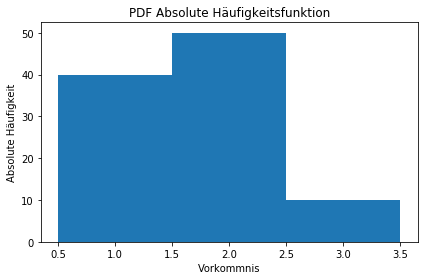
\includegraphics[height=2cm]{img/pdf1.png} \\
				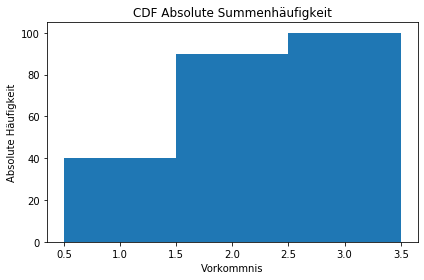
\includegraphics[height=2cm]{img/cdf1.png} \\
			\end{multicols*}
			
		\subsection{Quantil}   
			\begin{itemize}\itemsep0pt				
				\item wenn: $n\cdot q\%1 == 0 \rightarrow R_{q} = \dfrac{1}{2}(x_{n\cdot q}+x_{n\cdot q+1})$
				\item wenn: $n\cdot q\%1 <> 0 \rightarrow R_{q} = x_{n\cdot q+i}$ \\ mit i: zwischen 0 und 1 und n$\cdot$q+1 ganzzahlig
				\item $R_{0.25} = Q_{1}$
				\item $R_{0.5} = Q_{2} = \tilde{x}$ (Median)
				\item $R_{0.75} = Q_{3}$		
				\item $Q_{3} - Q_{1} = IQR$
			\end{itemize}
		\subsection{Boxplot}   
			\includegraphics[height=1.8cm]{img/Boxplot.png} \\
		\subsection{Varianz \& Standartabweichung}   
			\begin{itemize}\itemsep0pt				
				\item Vorkommnis: 1, 4, 7
				\item Varianz: $\sigma^{2} =  \dfrac{\Sigma(x_{i} -\bar{x})^{2}}{n} = \dfrac{9+0+9}{3} = 6$
				\item kor. Varianz: $\hat{\sigma}^{2} = \dfrac{\Sigma(x_{i} -\bar{x})^{2}}{n-1} = \dfrac{9+0+9}{2} = 9$
				\item Standartabweichung: $\sigma = \sqrt{6}$
				\item kor. Standartabweichung $\hat{\sigma} = \sqrt{9} = 3$
			\end{itemize}
		\section{Regression}
			\subsection{Lineare Regression}
				\begin{itemize}\itemsep0pt				
					\item $g(x) = mx + d$
					\item Steigung: $m = \dfrac{s_{xy}}{s_{xx}}$
					\item $d = \bar{y} - m\bar{x}$
					\item Kovarianz: $s_{xy} = \overline{x \cdot y} - \bar{x} \cdot \bar{y}$
					\item Varianz der x-Werte: $s_{xx} = \overline{x^{2}} - \bar{x}^{2}$
					\item Totale Varianz: $s_{y}^{2}=s_{yy} = \overline{y^{2}} - \bar{y}^{2}=  \dfrac{1}{n}\Sigma(y_{i}-\bar{y})^{2}$
					\item Residuenvarianz: $s_{\varepsilon}^{2} = s_{yy}-\dfrac{s_{xy}^{2}}{s_{xx}}$
					\item Summe der Residuen Quadrate: $s_{\varepsilon}^{2}\cdot n$
					\item Erklärte Varianz: $s_{\hat{y}}^{2}=s_{y}^{2}-s_{\varepsilon}^{2} $
					\item Bestimmtheitsmass: $R^{2}=\dfrac{s_{\hat{y}}^{2}}{s_{y}^{2}}$
					\item Pearson Korrelationskoeffizient: $R=r_{xy}=\dfrac{s_{xy}}{s_{x}s_{y}}$
					\item Korrigiertes X: $X_{kor} = \dfrac{X\cdot n}{n-1}$
				\end{itemize}
				
			\subsection{Korrelationskoeffizient $r_{xy}$}		
				\begin{itemize}\itemsep0pt				
					\item Pearson-Korrelationskoeffizient, auch Bravais-Pearson-Korrelation oder Produkt-Moment-Korrelation.
					\item Der Korrelationskoeffizient $r_{xy}$ ist so definiert, das seine Werte immer zischen -1 und +1 liegen, also $-1 \leq r_{xy} \leq +1$
					\item Je näher $r_{xy}$ bei -1 oder bei 1 liegt, umso besser liegen die Punkte ($x_{i}, y_{i}$) um eine Gerade konzentriert.
					\item $r_{xy} > 0$: Die Punkte liegen tendenziell um eine Gerade mit positiver Steigung (gleichsinniger linearer Zusammenhang, positive Korrelation).
					\item $r_{xy} < 0$: Die Punkte liegen tendenziell um eine Gerade mit negativer Steigung (gegensinniger linearer Zusammenhang, negative Korrelation).
					\item $r_{xy} \approx 0$: Kein linearer Zusammenhang zwischen den beiden Merkmalen.
				\end{itemize}				
				
			\subsection{Spearman-Rangkorrelation $r_{sp}$}		
				\begin{itemize}\itemsep0pt				
					\item Die Spearman-Rangkorrelation misst Stärke und Richtung des streng monotonen Zusammenhangs zwischen  zwei Merkmalen $x$ und $y$.
					\item Bei  der  Spearman-Korrelation  wird  nicht  davon ausgegangen,  dass  die  Daten  aus  einer bestimmten  Verteilung stammen,  es  handelt  sich  um  ein sogenanntes nichtparametrisches Korrelationsmass. 
				\end{itemize}		
					
				\subsubsection{Rang}		
					\begin{itemize}\itemsep0pt				
					\item $x_{i}: 12, 17, 6, 17, 23$
					\item $rg(x_{i}): 2, 3.5, 1, 3.5, 5$
					\item $\overline{rg(x)}: 3$
					\item $rg(x_{i})-\overline{rg(x)}: -1, 0.5, -2, 0.5, 2$
					\item $r_{sp}=\dfrac{\Sigma (rg(x_{i})-\overline{rg(x)})(rg(y_{i})-\overline{rg(y)})}{\sqrt{\Sigma (rg(x_{i})-\overline{rg(x)})^{2}} \cdot \sqrt{\Sigma (rg(y_{i})-\overline{rg(y)})^{2}}}$
				\end{itemize}
				
			 \subsection{Nichtlineares Verhalten}
			     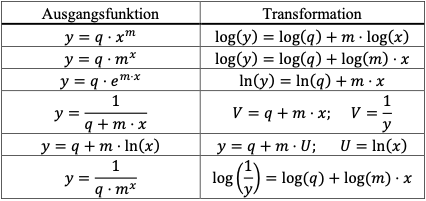
\includegraphics[height=3.25cm]{img/regression1.png} \\


		\section{Kombinatorik}
			\begin{itemize}\itemsep0pt				
				\item Binomialkoeffizient ${n\choose m} = \dfrac{n!}{(n-m)!\cdot m!}$
				\item Wenn jede der $n$ Stellen $m$ Zustände einnehmen kann, dann gibt es $m^{n}$ mögliche Kombinationen.
				\item Wenn aus $n$ unterschiedlichen Elementen $m$ mit \textbf{unbestimmter} Reihenfolge ausgewählt werden, dann gibt es ${n\choose m}$ mögliche Kombinationen.
				\item Wenn aus $n$ unterschiedlichen Elementen $m$ mit  \textbf{bestimmter} Reihenfolge ausgewählt werden, dann gibt es $\dfrac{n!}{(n-m)!}$ mögliche Kombinationen.
				\item Wenn aus $n$ unterschiedlichen \textbf{Kategorien} $m$ Elemente ausgewählt werden, dann gibt es ${n+m-1\choose m}$ mögliche Kombinationen.
			\end{itemize}
			
		\section{Kenngrössen}
			\begin{itemize}\itemsep0pt				
				\item $E(X) = \Sigma P(X=x)$
				\item $E(X+Y) = E(X) + E(Y)$
				\item $E(aX) = aE(X)$
				\item $V(X) = E(X) \cdot (x-E(X))^{2}$
				\item $V(X) = E(X^{2}) - (E(X))^{2}$
				\item $V(aX+b) = a^{2} \cdot V(X)$
			\end{itemize}
			
		\section{Intervallwahrscheinlichkeiten}		
			\begin{itemize}\itemsep0pt				
				\item $P(X \leq b) = \int_{-\infty}^b f(u)\delta u$
				\item $P(a < X \leq b) = \int_{-\infty}^b f(u)\delta u - \int_a^\infty f(u)\delta u =  \int_a^b f(u)\delta u $
				\item $P(X > a) = \int_a^\infty f(u)\delta u$
			\end{itemize}	
			
		\section{Diskrete Verteilungen}
			
			\subsection{Hypergeometrische Verteilung}
				\begin{itemize}\itemsep0pt			
					\item $X \sim H(N,M,n)$
					\item $N$ Objekteanzahl, $M$ Merkmalsträger, $n$ Ziehungsanzahl
					\item $P(X=x)=\dfrac{{M\choose x} \cdot {N-M\choose n-x}}{{N\choose n} }$
					\item Lotto: $P(X=x)=\dfrac{{6\choose x} \cdot {49-6\choose 6-x}}{{49\choose 6} }$
					\item $N$ Kugeln, $M$ schwarz, ohne Zurücklegen $n$ ziehen. Wahrscheinlichkeit für $x$ schwarze Kugeln $P(X=x)$
					\item $E(X) = n \cdot \dfrac{M}{N}$
					\item $V(X) = n \cdot \dfrac{M}{N} (1-\dfrac{M}{N})\dfrac{N-n}{N-1}$
				\end{itemize}	
			
			\subsection{Bernoulliverteilungverteilung}
				\begin{itemize}\itemsep0pt				
					\item Bernoulli-Experimente sind Zufallsexperimente mit nur zwei möglichen Ergebnissen (0/1)
					\item $P(X=1)=p$
					\item $P(X=0)=1-p=q$
					\item $E(X)=p$
					\item $V(X)=p\cdot q$
				\end{itemize}	
			
			\subsection{Binomialverteilung}
				\begin{itemize}\itemsep0pt				
					\item $X \sim B(n,p)$
					\item $q = 1-p$
					\item n-faches Bernoulli-Experiment
					\item $P(X=x)={n\choose x} \cdot p^{x} \cdot q^{n-x} $
					\item $E(X)=n\cdot p$
					\item $V(X)=n\cdot p\cdot q$
				\end{itemize}	
				
				\subsubsection{Binomialverteilung als Näherung der hypergeometrischen Verteilung}
					\begin{itemize}\itemsep0pt				
						\item Faustregel: $n \lesssim \dfrac{N}{20}$
						\item $H(N,M,n) \approx B(n,\dfrac{M}{N})$
						\item $N$ Einheiten, $M$ Merkmalsträger, Stichprobengrösse $n$
					\end{itemize}	
			
			\subsection{Poissonverteilung}
				\begin{itemize}\itemsep0pt				
					\item $X \sim Poi(\lambda)$
					\item Beschreibt die Anzahl Ereignisse pro Zeit, Fläche, Länge,...
					\item $P(X=x)= \dfrac{\lambda^{x}}{x!}e^{-\lambda}, \lambda > 0$
					\item $E(X)= \lambda$
					\item $V(X)= \lambda$
					\item $V(X)= \lambda$
				\end{itemize}	
				
				\subsubsection{Poissonverteilung als Näherung der Binomialverteilung}
					\begin{itemize}\itemsep0pt				
						\item Faustregel: $n \gtrsim 50$, $p \lesssim 0.1$
						\item $B(n,p) \approx Poi(n\cdot p)$
						\item $N$ Einheiten, $M$ Merkmalsträger, Stichprobengrösse $n$
					\end{itemize}	
			
		\section{Stetige Verteilungen}
			\subsection{Gaussverteilung/Normalverteilung}
				\begin{itemize}\itemsep0pt				
					\item $X \sim N(\mu ;\sigma )$
					\item Standardnormalverteilung $N(0;1)$
					\item $U=\dfrac{X-\mu}{\sigma}$
					\item $P(X\leq x)= P(U \leq \dfrac{x-\mu}{\sigma}) = \phi(u)=$ Tabellenwert
					\item $E(X)=\mu$
					\item $V(X)=\sigma^{2}$
					\item Ca. 68 \% der beobachteten Werte liegen zwischen $\mu - \sigma$ und $\mu + \sigma$.
					\item Ca. 95 \% der beobachteten Werte liegen zwischen $\mu - 2\sigma$ und $\mu + 2\sigma$.
					\item Ca. 99.7 \% der beobachteten Werte liegen zwischen $\mu - 3\sigma$ und $\mu + 3\sigma$.
				\end{itemize}	
				
				\subsubsection{Normalverteilung als Näherung der Binomialverteilung}		
					\begin{itemize}\itemsep0pt				
						\item Faustregel: $npq > 9$
						\item $\mu = np$
						\item $\sigma = npq$
						\item $X \sim B(n;p)$
						\item $Y \sim N(\mu;\sigma)$
						\item $P(a\leq X \leq b) = P((a-1) < X < (b-1)) $
						\item $P(a\leq X \leq b) \approx P((a-0.5) < Y < (b+0.5)) $
					\end{itemize}			
				
			\subsection{Zentraler Grenzwertsatz}
			 Identisch verteilte und stochastisch unabhängige Zufallsvariablen:
			 \begin{itemize}\itemsep0pt				
					\item $E(S_{n})=n\cdot \mu$
					\item $V(S_{n})=n\cdot \sigma^{2}$
					\item $E(\bar{X}_{n})=\mu$
					\item $V(\bar{X}_{n})=\dfrac{\sigma^{2}}{n}$
					\item $S_{n} \sim N(n\cdot \mu ;\sqrt{n}\cdot \sigma )$
					\item $\bar{X}_{n}  \sim N(\mu ; \dfrac{\sigma}{\sqrt{n}} )$
				\end{itemize}	
				
			\section{Schliessende Statistik}
			
			 	\begin{itemize}\itemsep0pt				
					\item Schätzfunktion $\Theta$ eines Parameters $\theta$ erwartungstreu: $E(\Theta)=\theta $
					\item Erwartungstreue Schätzfunktion $\Theta_{1}$ effizienter $\Theta_{2}$: $ V(\Theta_{1})<V(\Theta_{2})$
					\item Konsistent $E(\Theta)\rightarrow\theta$ und $V(\Theta)\rightarrow 0$ für $n\rightarrow \infty$
				\end{itemize}	
				\subsection{Schätzfunktionen für die wichtigsten statistischen Parameter}
					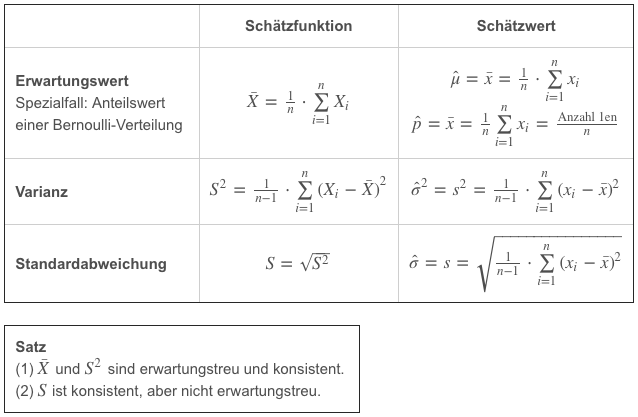
\includegraphics[height=6cm]{img/schaetz1.png} 



\end{multicols*}

\begin{multicols*}{2}
\setlength{\columnseprule}{0.4pt}

\section{Tabellen}
	\subsection{CDF $\Phi$(u) der Standardnormalverteilung}

		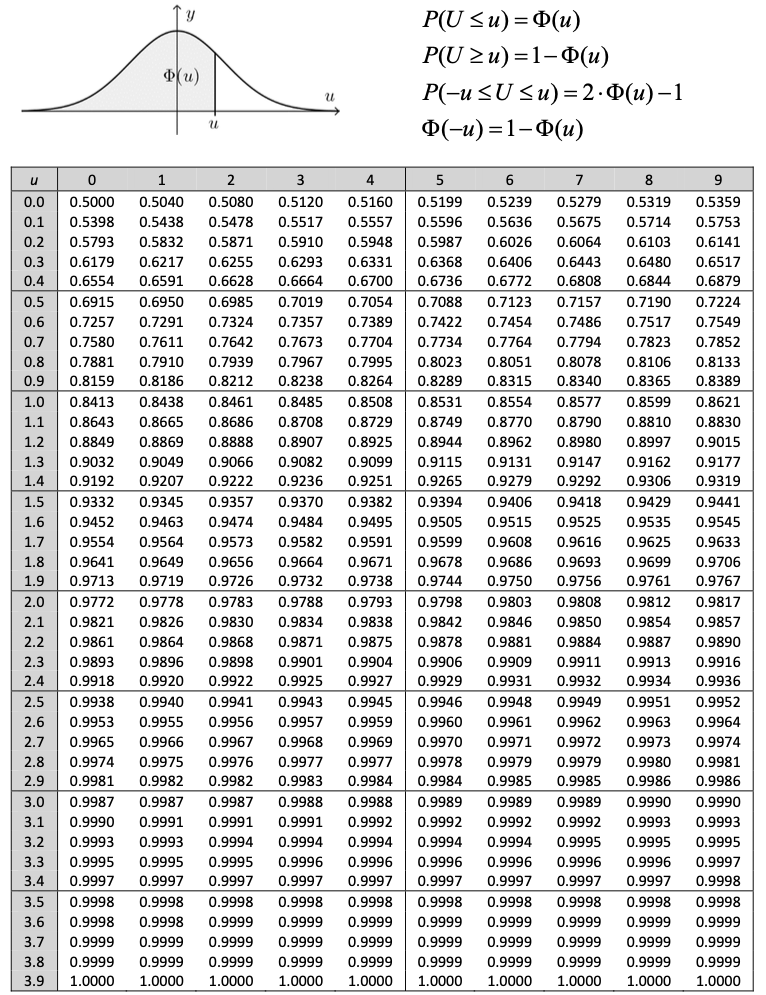
\includegraphics[height=17.75cm]{img/Standardnormalverteilung.png}

	\subsection{Quantile der Standardnormalverteilung}

		\begin{multicols*}{2}
			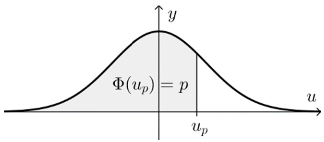
\includegraphics[height=3cm]{img/Quantile_Standardnormalverteilung1.png}
			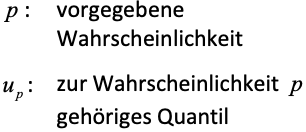
\includegraphics[height=1.5cm]{img/Quantile_Standardnormalverteilung2.png} \\
			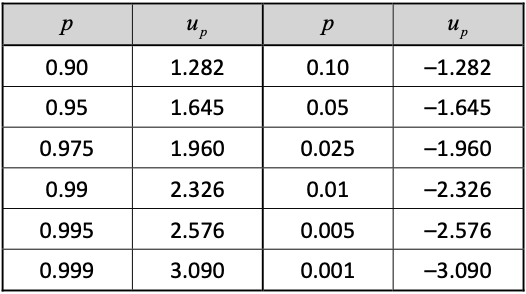
\includegraphics[height=3.75cm]{img/Quantile_Standardnormalverteilung3.png}
		\end{multicols*}

	\subsection{Quantile der t‐Verteilung}
		\begin{multicols*}{2}
			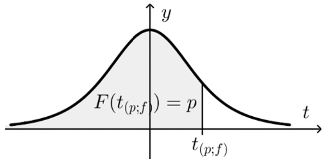
\includegraphics[height=3cm]{img/QuantileT1.png}
			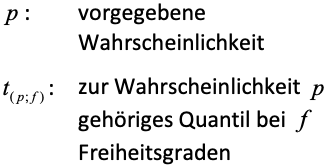
\includegraphics[height=2cm]{img/QuantileT2.png} \\
			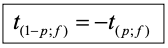
\includegraphics[height=1cm]{img/QuantileT3.png} \\
			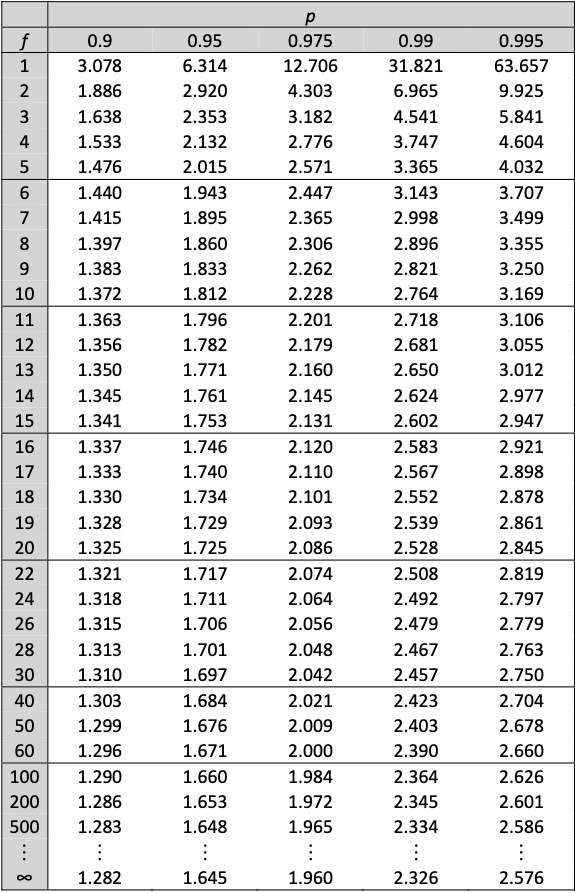
\includegraphics[height=10cm]{img/QuantileT4.png}
		\end{multicols*}

	\subsection{Quantile der Chi‐Quadrat‐Verteilung}
		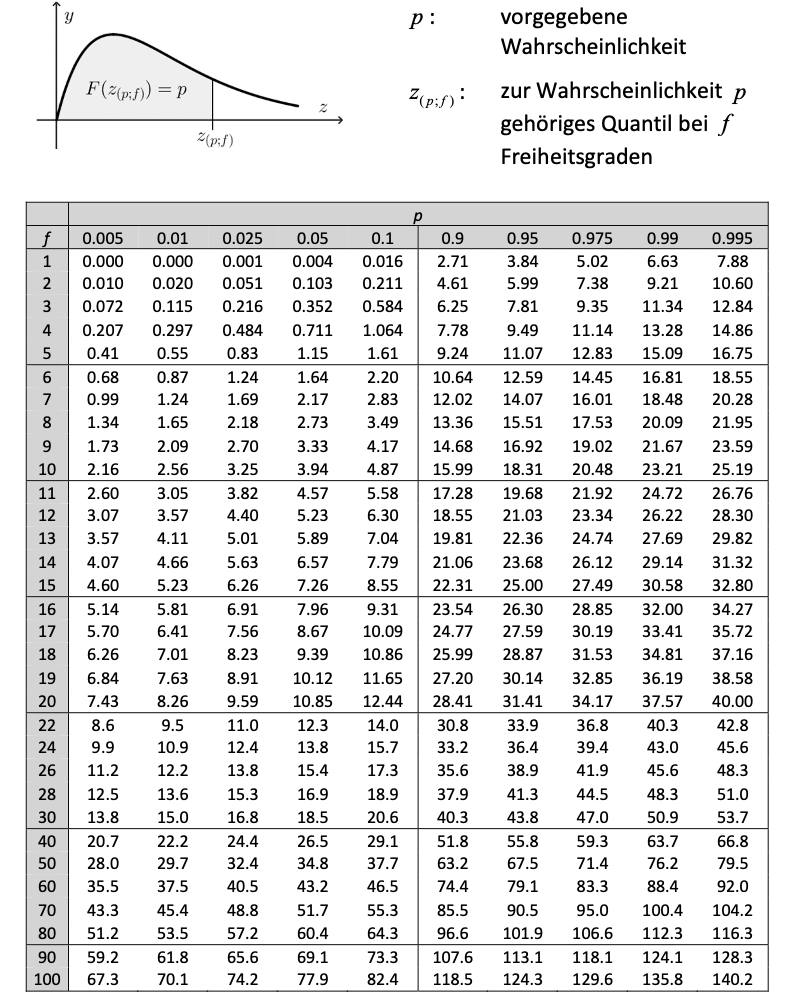
\includegraphics[height=18cm]{img/QuantileChi.png}

\end{multicols*}
% Dokumentende % ======================================================================
\end{document}